\printedpage{120}
% head: A. Grothendieck : Dérivateurs, Ch. XII, Édition des Universités de Montpellier II et Paris VII

\msp{page 180}
$\mathrm{b}_n \Longrightarrow \mathrm{c}_n$. We can suppose that $f$ is a Hot-fibration (and even Hot-perfect if we feel like it \dots). We already know that for
\[
H^i(Y,F) \longrightarrow H^i(X,f^*F) \tag*{$(*)$}
\]
everything is O.K. if $i \in \{0,1\}$. So we can suppose $F$ abelian. If that gets us anywhere, we can suppose, by induction, (that the implication $\mathrm{b}_{n-1} \Longrightarrow \mathrm{c}_{n-1}$ is known, hence) that $(*)$ is \texttt{[an]} isomorphism for $i<n$. Remains to see it for $i=n$. We are reduced of course, since $\pi_0(f)$ is bijective, to the case where $X$, $Y$ are 0-connected, so there is essentially a single fiber $Z$. The homotopy exact sequence tells us that
\[
\pi_i(Z,z)=0 \qquad \text{for } i \le n-1 \ (Z \text{ is } (n-1)\text{-connected})
\]
and moreover
\[
\pi_n(Z,z) \longrightarrow \pi_n(X,z) \qquad \text{is zero}
\]
(since $\pi_n(X,z) \longrightarrow \pi_n(Y,y)$ \texttt{[is an]} isomorphism hence \texttt{[a]} monomorphism), so
\[
\pi_{n+1}(Y,y) \longrightarrow \pi_n(Z,z) \qquad \text{\texttt{[is an]} epimorphism.}
\]
As $Z$ is $(n-1)$-connected (hence also 1-connected), we have
\[
H^i(Z,G)=0\ , \qquad \text{if } 0<i<n\ , \tag*{$(*)$}
\]
for $G$ locally constant (hence constant) on $Z$.

\msp{page 181}
Let us write the Leray spectral sequence for $f : X \longrightarrow Y$ and $f^*F = F_X$:
\[
H^*(X,f^*F) \Longleftarrow E_2^{pq} = H^p(Y,H^q(Z,f^*F)),
\]
where ``$H^q(Z)$'' is to be viewed as a local system on $Y$. So by $(*)$ we have
\[
E_2^{pq}=0 \qquad \text{if } 0<q<n, \qquad
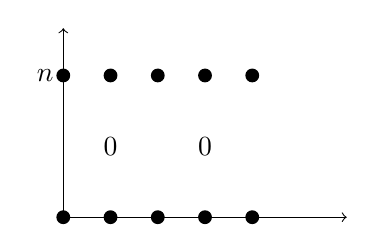
\begin{tikzpicture}[baseline=0pt, x=0.6cm, y=0.6cm]
\draw[->] (0,0) -- (0,4);
\draw[->] (0,0) -- (6,0);
\node[left] at (0,3) {$n$};
\foreach \i in {0,...,4} { \fill (\i,3) circle (2.5pt); \fill (\i,0) circle (2.5pt); }
\node at (1,1.5) {$0$};
\node at (3,1.5) {$0$};
\end{tikzpicture}
\qquad ,
\]
so we find the exact sequence
\[
0 \longrightarrow H^n(Y,F) \longrightarrow H^n(X,F_X) \xrightarrow{\ \alpha\ } H^0(Y,\ \underbrace{H^n(Z,\overbrace{F_Z}^{M_Z})}_{\begin{array}{l}\scriptstyle = \ \mathrm{Hom}(\pi_n(Z,z),M)\\ \scriptstyle \text{by \texttt{[the]} Hurewicz thm.}\end{array}}\ ) \longrightarrow H^{n+1}(Y,F).
\]

\printedpage{121}
% head: A. Grothendieck : Dérivateurs, Ch. XII, Édition des Universités de Montpellier II et Paris VII

Here I fix a point $x$ of $X$, $Z$ denotes the fiber of $f$ at $y=f(x)$, and $M$ that of $F$ at $y$, $M=F_y$. The group $\pi_1(Y)$ acts on it, for that matter $\pi \overset{\text{def}}{=} \pi_1(X,x) \simeq \pi_1(Y,y)$ does too. The $H^0(Y,H^n(Z,F_Z))$ can be interpreted, unless I am mistaken, as
\[
\mathrm{Hom}_\pi(\pi_n(Z,x),M),
\]
taking into account the action of $\pi=\pi_1(X,x)$ on $\pi_n(Z,x)$ as well. (To be checked.) We have to interpret the arrow
\[
H^n(X,F_X) \longrightarrow \mathrm{Hom}_\pi(\pi_n(Z,x),M),
\]
via the composite map \texttt{[where $z=x$, viewed as a point of $Z$]}
\[
\pi_n(Z,z) \longrightarrow \pi_n(X,x) \longrightarrow H_n(X,\mathbf{Z}). \tag*{$(*)$}
\]
If $F$ is \textit{constant} on $Y$ (e.g. if $Y$ \texttt{[is]} 1-connected), thus with value $M$, we have the canonical arrows
\[
H^n(X,F_X) = H^n(X,M) \longrightarrow \mathrm{Hom}(H_n(X,\mathbf{Z}),M) \longrightarrow \mathrm{Hom}(\pi_n(Z,z),M)\text{(\footnotemark[118])} \tag*{$(*')$}
\]
\footnotetext[118]{thanks to composition with $(*)$.}
\texttt{[read: }$\mathrm{Hom}_\pi$\texttt{]},

\msp{page 182}
and surely (apart from any hypothesis of type $\mathrm{b}_n$ or other) the direct canonical map ``of localization on $Y$'', followed by \dots,
\[
H^n(X,F_X) \longrightarrow H^0(Y,H^n(Z,F_Z)) \longrightarrow \mathrm{Hom}_\pi(\pi_n(Z),M) \tag*{$(**)$}
\]
is none other than the composite of the canonical maps above. In the present case where we suppose $\mathrm{b}_n$, the second arrow in $(**)$ is \texttt{[an]} isomorphism, so the composite ``is none other'' than the localization arrow itself. On the other hand $\pi_n(Z,z) \longrightarrow \pi_n(X,x)$ in $(*)$ is zero, so also $\pi_n(Z,z) \longrightarrow H_n(X,\mathbf{Z})$, so also the composite arrow $(*')$ deduced from it. Let us then return to the Leray exact sequence (previous page), we find that $H^n(Y,F) \xrightarrow{\ \sim\ } H^n(X,F_X)$.

How to recover the case where $F$ is \textit{not} constant? In the case $n=2$, this worked, by passing to the universal covers $\tilde{X}$, $\tilde{Y}$ of $X$, $Y$ (with respect to the chosen points $x$, $y$), and writing the spectral sequences
\[
\begin{tikzcd}[row sep=small, column sep=small]
H^*(Y,F) \arrow[d] & \Longleftarrow & E_2^{pq} \arrow[d] & = & H^p(\pi,H^q(\tilde{Y},F_{\tilde{Y}})) \\
H^*(X,F_X) & \Longleftarrow & E^{\prime pq}_2 & = & H^p(\pi,H^q(\tilde{X},F_{\tilde{X}})).
\end{tikzcd}
\]
The hypothesis $\mathrm{b}_n$ is preserved in passing from $f : X \longrightarrow Y$ to $\tilde{f} = \tilde{f}_x : \tilde{X} \longrightarrow \tilde{Y}$, so we know that
\printedpage{122}
% head: A. Grothendieck : Dérivateurs, Ch. XII, Édition des Universités de Montpellier II et Paris VII
\msp{page 183}
\[
E_2^{pq} \xrightarrow{\ \sim\ } E^{\prime pq}_2 \qquad \text{\texttt{[is an]} isomorphism if } q \le n. \tag*{$(*)$}
\]
In the case $n=2$, using that
\[
E_2^{p1} = E^{\prime p1}_2 = 0 \qquad \text{since } H^1(\tilde{X}) = H^1(\tilde{Y}) = 0, \qquad
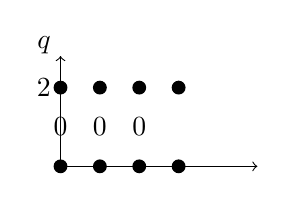
\begin{tikzpicture}[baseline=0pt, x=0.5cm, y=0.5cm]
\draw[->] (0,0) -- (0,2.8);
\draw[->] (0,0) -- (5,0);
\node[above left] at (0,2.6) {$q$};
\node[left] at (0,2) {$2$};
\foreach \i in {0,...,3} { \fill (\i,2) circle (2.5pt); \fill (\i,0) circle (2.5pt); }
\node at (0,1) {$0$};
\node at (1,1) {$0$};
\node at (2,1) {$0$};
\end{tikzpicture}
\qquad ,
\]
we find two exact sequences
\[
\begin{tikzcd}
0 \arrow[r] & H^2(\pi,H^0(\tilde{Y})) \arrow[r] \arrow[d, "\text{iso}"] & H^2(Y) \arrow[r] \arrow[d] & H^0(\pi,H^2(\tilde{Y})) \arrow[r] \arrow[d, "\text{iso}"] & H^3(\pi,H^0(\tilde{Y})) \arrow[d, "\text{iso}"] \\
0 \arrow[r] & H^2(\pi,H^0(\tilde{X})) \arrow[r] & H^2(X) \arrow[r] & H^0(\pi,H^2(\tilde{X})) \arrow[r] & H^3(\pi,H^0(\tilde{X})),
\end{tikzcd}
\]
and a homomorphism from one to the other, which allows us to conclude by the 5 lemma that $H^2(Y,F) \longrightarrow H^2(X,F_X)$ is \texttt{[an]} isomorphism. But for arbitrary $n$, the relation $(*)$ on the $E_2$ terms (for $q \le n$) does not seem to me to imply the similar relation for the higher $E_n$, and from there for the $E_\infty$ terms, which would allow us to conclude.

So I return to the exact sequence p. 181, with $F$ a sheaf that is \textit{twisted.} I feel like finding a canonical map
\[
H^n(X,G) \longrightarrow \overbrace{\mathrm{Hom}_\pi(\pi_n(X,x),G_x)}^{\text{\scriptsize Homs \textit{additive} of course, i.e. of $\mathbf{Z}[\pi]$-modules}} \qquad ,
\]
where $G$ is any locally constant abelian sheaf on $X$, and $\pi = \pi_1(X,x)$. If I interpret
\msp{page 184}
$\pi_n(X,x)$ in terms of homotopy classes of pointed maps
\[
(S^n,x_0) \xrightarrow{\ \varphi\ } (X,x)
\]
I do have, for such a map $\varphi$,
\[
\varphi^* : H^n(X,G) \longrightarrow H^n(S^n,\ \overbrace{\varphi^*G}^{\simeq\,(G_x)_{S^n}}\ ) \simeq G_x
\]
(taking into account that $S^n$ is 1-connected, and that its $n$-cohomology with values in a constant sheaf $M$ is $M$.) Surely the map
\[
H^n(X,G) \longrightarrow G_x
\]
\printedpage{123}
% head: A. Grothendieck : Dérivateurs, Ch. XII, Édition des Universités de Montpellier II et Paris VII
thus defined depends only on the pointed homotopy class of $\varphi$, hence
\[
\pi_n(X,x) \times H^n(X,G) \longrightarrow G_x,
\]
and we must also prove a) that this is compatible with the actions of $\pi = \pi_1(X,x)$, and b) that it is additive in $\pi_n(X,x)$, to have the desired map
\[
H^n(X,G) \longrightarrow \mathrm{Hom}_\pi(\pi_n(X,x),G_x).
\]
If I admit this, it is only one step to admitting also that the arrow that really interests us (in the exact sequence p. 181)
\msp{page 185}
\[
H^n(X,F_X) \longrightarrow \mathrm{Hom}_\pi(\pi_n(Z,z),\underbrace{M}_{=\,F_y})
\]
is none other than the composite of the preceding arrow (previous page) for $G = F_X$, with
\[
\mathrm{Hom}_\pi(\pi_n(X,x),M) \longrightarrow \mathrm{Hom}_\pi(\pi_n(Z,x),M)
\]
deduced from
\[
\pi_n(Z,x) \longrightarrow \pi_n(X,x).
\]
Now this arrow is zero, by the hypothesis $\mathrm{b}_n$. So the arrow $\alpha$ in the exact sequence page 181 is zero, so $H^n(Y,F) \longrightarrow H^n(X,F_X)$ is \texttt{[an]} isomorphism, q.e.d. (but there is quite a bit of checking to do \dots).

$\mathrm{c}_n \Longrightarrow \mathrm{a}_{n-1}$. We can proceed by induction on $n$. (NB The statement makes sense even for $n=1$, where it is proved, and even $\mathrm{c}_1 \Longrightarrow \mathrm{b}_1$, and $\mathrm{b}_1 \Longrightarrow \mathrm{a}_0$, more generally $\mathrm{b}_n \Longrightarrow \mathrm{a}_{n-1}$, immediate from \texttt{[the]} homotopy exact sequence.) So we already know, in addition to the hypothesis $\mathrm{c}_n$, that we have $\mathrm{a}_{n-2}$, i.e. $Z$ is $(n-2)$-connected. We have to prove that it is even $(n-1)$-connected, i.e. $\pi_{n-1}(Z)=0$. The case $n=2$ requires % [sic] L’enoncé -> L’énoncé, missing accent on é
\msp{page 186}
perhaps special attention, since we do not even know yet that $Z$ is 1-connected. But we know that $\mathrm{c}_2$ implies $\mathrm{c}_1$, which is equivalent \texttt{[?]} to $\mathrm{b}_1$, so we have
\[
\pi_1(X,x) \longrightarrow \pi_1(Y,y) \qquad \text{isomorphism,}
\]
so
\[
\pi_1(Z,x) \longrightarrow \pi_1(X,x) \qquad \text{\texttt{[is]} \textit{zero,}}
\]
so
\[
\pi_2(Y,y) \longrightarrow \pi_1(Z,x) \qquad \text{\texttt{[is an]} epimorphism,}
\]
which implies at least that $\pi_1(Z,x)$ is \textit{abelian.} We must view it as a $\pi$-module, and prove its vanishing as such (using $\mathrm{c}_2$).

\printedpage{124}
% head: A. Grothendieck : Dérivateurs, Ch. XII, Édition des Universités de Montpellier II et Paris VII

Let us pass to the general case. We have for $F$ locally constant abelian on $Y$
\[
H^*(X,F_X) \Longleftarrow \underbrace{E_2^{pq} = H^p(Y,H^q(Z,F_Z))}_{\begin{array}{l}\scriptstyle = 0 \text{ if } 0<q<n-1\\ \scriptstyle \text{since } Z \text{ is } (n-2)\text{-connected}\end{array}}, \qquad
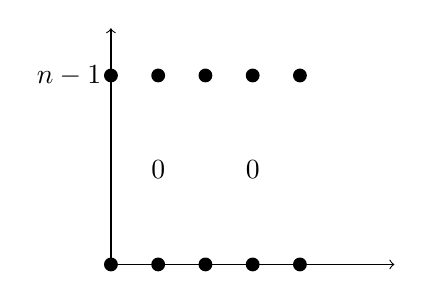
\begin{tikzpicture}[baseline=0pt, x=0.6cm, y=0.6cm]
\draw[->] (0,0) -- (0,5);
\draw[->] (0,0) -- (6,0);
\node[left] at (0,4) {$n-1$};
\foreach \i in {0,...,4} { \fill (\i,4) circle (2.5pt); \fill (\i,0) circle (2.5pt); }
\node at (1,2) {$0$};
\node at (3,2) {$0$};
\end{tikzpicture}
\qquad ,
\]
Hence
\[
0 \longrightarrow H^{n-1}(Y,F) \longrightarrow H^{n-1}(X,F_X) \longrightarrow \underbrace{H^0(Y,H^{n-1}(Z,F_Z))}_{\begin{array}{l}\scriptstyle \mathrm{Hom}_\pi(\pi_{n-1}(Z,x),F_x)\\ \scriptstyle \text{by Hurewicz}\end{array}} \longrightarrow H^n(Y,F) \longrightarrow H^n(X,F_X).
\]
The hypothesis $\mathrm{c}_n$ implies that we have
\msp{page 187}
\[
\mathrm{Hom}_\pi(\pi_{n-1}(Z,x),\underbrace{M}_{=\,F_x}) = 0
\]
and this \textit{whatever the $\pi$-module $M$,} since $\pi = \pi_1(X,x) \xrightarrow{\ \sim\ } \pi_1(Y,y)$. This implies (taking e.g. $M = \pi_{n-1}(Z,x)$!) that $\pi_{n-1}(Z,x)=0$. (But keeping in mind, in the case $n=2$, that we already know that $\pi_1(Z,x)$ is abelian).

So the theorem corrected on page 178 does look true. It is a bit sad, since in each of the implications % [sic] rectifie -> rectifié, past participle intended
\[
\mathrm{a}_n \ \Longrightarrow\ \mathrm{b}_n \ \Longrightarrow\ \mathrm{c}_n \ \Longrightarrow\ \mathrm{a}_{n-1}
\]
we lose a smidgen, and in the end we come out with the magnificent implication
\[
\mathrm{a}_n \ \Longrightarrow\ \mathrm{a}_{n-1}.
\]
In any case, it is $\pm$ clear that the ``right'' localizer $W_n$, the one that is to define the ``$n$-homotopy types'' as objects of $\mathrm{Hot}_{W_n}$, is defined by the condition $\mathrm{a}_n$.

\section*{2\quad Criterion for $W_n$-asphericity.}

I am going to try to do better when $Y$ is reduced to a point. This time, I